\documentclass[10pt]{beamer}

\usetheme[progressbar=frametitle]{metropolis}

\usepackage{booktabs}
\usepackage[scale=2]{ccicons}

\usepackage{pgfplots}
\usepgfplotslibrary{dateplot}

\usepackage{xspace}
\newcommand{\themename}{\textbf{\textsc{metropolis}}\xspace}

\title{BioComputers}
% \subtitle{A modern beamer theme}
\date{\today}
\author{Vinod Kumar S}
\institute{College of Engineering Trivandrum}
\titlegraphic{\hfill
\includegraphics[height=1.5cm]{logo}}

\begin{document}

\maketitle

\begin{frame}{Table of contents}
  \setbeamertemplate{section in toc}[sections numbered]
  \tableofcontents[hideallsubsections]
\end{frame}

\section{Introduction}

\begin{frame}[fragile]{What is DNA ?}
  \begin{itemize}
      \item{DNA or deoxyribonucleic acid is made up of molecules called nucleotides.}
      \item{Each nucleotide contains a phosphate group, a sugar group and a nitrogen base.}
      \item{The four types of nitrogen bases are adenine (A), thymine (T), guanine (G) and cytosine (C).}
      \item{The order of these bases is what determines DNA's instructions, or genetic code.}
      \item{ Bond in pairs
          \begin{itemize}
        \item A - T
                \item C - G 
      \end{itemize}}
  \end{itemize}
\end{frame}

\begin{frame}{DNA Structure}
  \begin{figure}
      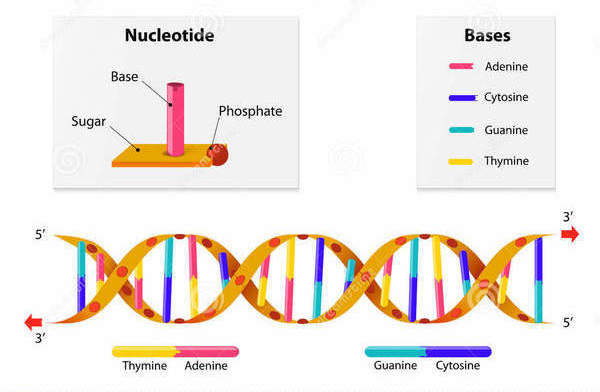
\includegraphics[width=\textwidth]{dna}   
  \end{figure}
\end{frame}

\begin{frame}[fragile]{What is BioComputers ?}
         \begin{itemize}
      \item{Biocomputers use systems of biologically derived molecules—such as DNA and proteins—to perform computational calculations involving storing, retrieving, and processing data.}
            \item{These computers use DNA to store information and perform complex calculations. DNA has a vast amount of storage capacity.}
            \item{ Computers might tap the vast storage capacity that enables DNA to hold the complex blueprints of living organisms.}
            \item{The storage capacity of a single gram of DNA can hold as much information as one trillion compact discs.}
    \end{itemize}
\end{frame}

\begin{frame}[fragile]{Can DNA Compute?}
         \begin{itemize}
      \item DNA itself doesnot carry out computations
      \item It rather acts as a massive memory
            \item But, the way complementary bases react with each other can be used to         compute things
            \item Proposed by Leonard Adleman - Inventor of Biological Computers in 1994
    \end{itemize}
\end{frame}

\begin{frame}[fragile]{Hamiltanion Path Problem}
  \begin{figure}
             \includegraphics[width=\textwidth]{hpp} 
  \end{figure}
    Determine whether there is a hamiltonian path from Boston to New York
\end{frame}

\begin{frame}[fragile]{Solving HPP using DNA}
  \begin{itemize}
    \item Encode this graph in a DNA
        \item{  Vertices are assigned a random DNA sequence 
          \begin{itemize}
        \item Boston = GCTACG
        \item San Diego = CTAGTA
      \end{itemize}}
         \item{  Edges are formed by concatenating $2^{nd}$ half of the originating city and $1^{st}$ half of the destination city and taking the complement
          \begin{itemize}
        \item Boston-San Diego = TGCGAT
      \end{itemize}}
            \item Use Polymerase Chain Reaction (PCR) to replicate the DNA with the correct start and end city
  \end{itemize}
\end{frame}

\begin{frame}[fragile]{Solving HPP using DNA}
  \begin{itemize}
        \item Put one primer on Boston and one on New York
    \item The right answer is replicated exponentially while wrong paths are replicated linearly or not at all
         \item Use \textit{gel elecrophoresis} to identify molecules with the right length
         \item Finally use \textit{affinity seperation} to weed out paths without all the cities
         \item If any DNA is left in the test tube, it is the Hamiltonian Path 
  \end{itemize}
\end{frame}

\section{Bio Computers}
\begin{frame}[fragile]{DNA Data Storage}
\begin{itemize}
  \item DNA is a good storage medium because data can be written into molecules more densely than the basic elements of conventional storage technologies can pack it in
    \item IDC predicts that the worldwide total of stored digital data will hit 16 trillion gigabytes next year, most of it housed in huge data centers
    \item It is estimated that a shoebox worth of DNA could hold the equivalent of roughly 100 giant data centers
    \item DNA can also be remarkably durable, particularly when kept cool and dry
\end{itemize}
\end{frame}

 \begin{frame}[fragile]{DNA Data Storage}
  \begin{figure}
        \includegraphics[width=0.8\textwidth]{dna-storage} 
  \end{figure}
    The pink smear in this test tube is DNA that has been synthesized to store digital data for long-term storage. Microsoft used the same technique to store roughly 200 megabytes of data
\end{frame}

\begin{frame}[fragile]{DNA Data Storage System - Write Operation}
   \begin{itemize}
    \item Storing data in DNA requires translating the 1s and 0s of binary digital files into long strings of the four different nucleotides, or bases, that make up DNA strands and write out the genetic code
  \end{itemize}
  \begin{figure}
        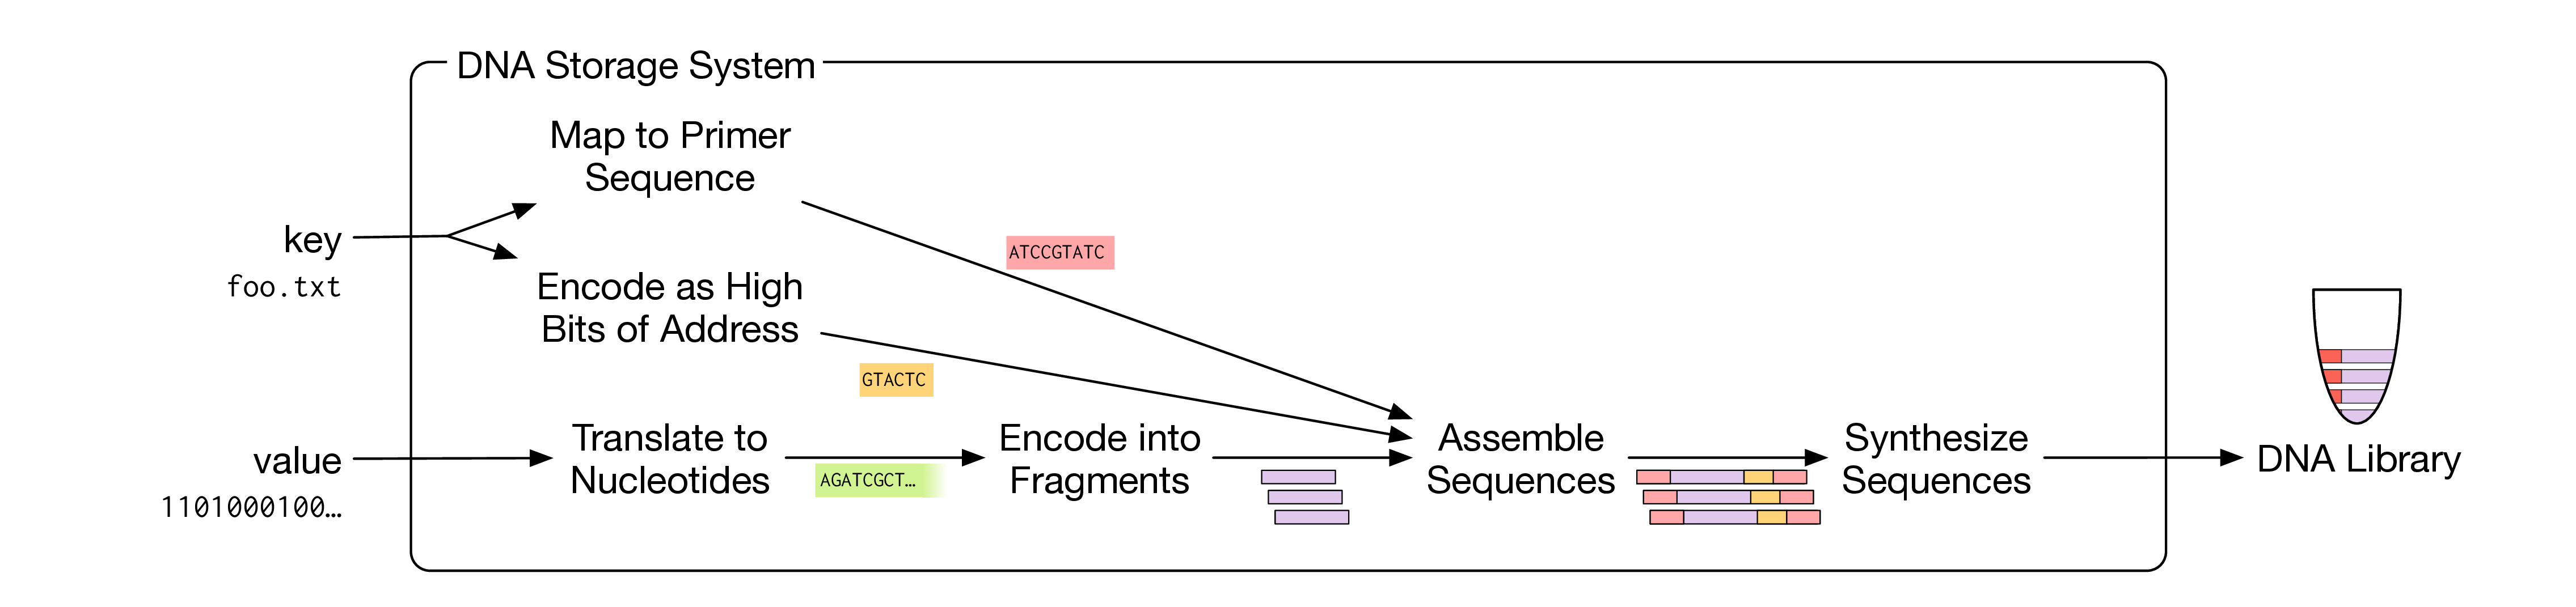
\includegraphics[width=\textwidth]{write} 
  \end{figure}
    The write process performs put(key, value), generating a DNA library.
\end{frame}

\begin{frame}[fragile]{DNA Data Storage System - Read Operation}
  \begin{figure}
        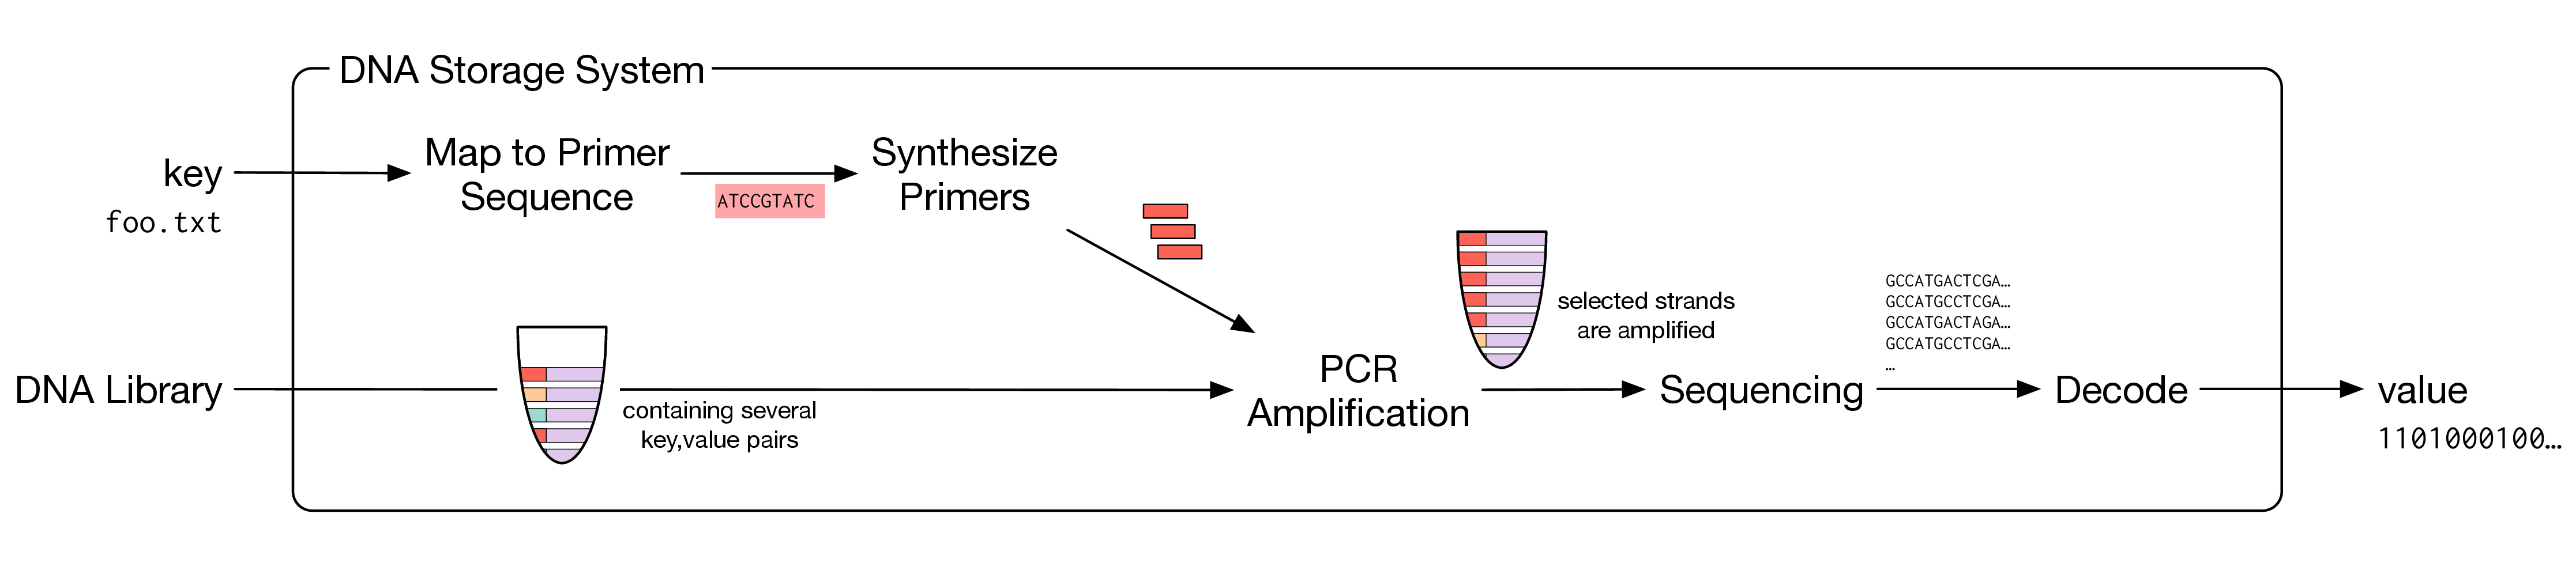
\includegraphics[width=\textwidth]{read} 
  \end{figure}
   The read process performs get(key) on a DNA library, returning the value
\end{frame}

\begin{frame}[fragile]{Transcriptor - Biological transistor }
  \begin{itemize} 
  
  \item Biological transistor the “transcriptor" is made from genetic material — DNA and RNA 
  \item  A transcriptor controls the flow of a specific protein, RNA polymerase, as it travels along a strand of DNA
  \item The creation of the transcriptor allows engineers to compute inside living cells to record
  \item Using transcriptors, logic gates can be created that can derive true-false answers to virtually any biochemical question that might be posed within a cell
  \item Transcriptor-based logic gates as “Boolean Integrase Logic,” or “BIL gates” for short
  
  \end{itemize}
\end{frame}

\begin{frame}[fragile]{Transcriptor - Biological transistor }
  \begin{itemize} 
  \item The BIL gates can test whether a given cell had been exposed to any number of external stimuli — the presence of glucose and caffeine, for instance
  \item BIL gates can then tell the cell to start or stop reproducing if certain factors were present
  \item  By coupling BIL gates with the team’s biological Internet, it is possible to communicate genetic information from cell to cell to orchestrate the behavior of a group of cells
  \item The BIL gates also provide signal amplification
  \end{itemize}
\end{frame}

\begin{frame}{Similarities between Conventional and Bio Computers}
  \begin{itemize}
        \item {Transformation of Data
          \begin{itemize}
        \item Both DNA computers and electronic computers use Boolean logic (AND, OR, NAND, NOR) to transform data.
                \item The logical command "AND" is performed by separating DNA strands according to their sequences, and the command "OR" is done by pouring together DNA solutions containing specific sequences.
      \end{itemize}
            }
             \item {Manipulation of Data
          \begin{itemize}
        \item Electronic computers and DNA computers both store information in strings, which are manipulated to do processes. 
      \end{itemize}
            }
            \item {Computation Ability
              \begin{itemize}
          \item All computers manipulate data by addition and subtraction. 
                    \item A DNA computer should be able to solve a satisfiability problem with 70 variables and 1,000 AND-OR connections. 
        \end{itemize}
            }
  \end{itemize}
\end{frame}
\begin{frame}{Differences between Conventional and BioComputers}
  \begin{table}
%     \caption{Largest cities in the world (source: Wikipedia)}
    \begin{tabular}{lr}
      \toprule
      Conventional & BioComputers \\
      \midrule
      Inorganic eg.Silicon & Biological eg.DNA \\ \\
      Sequential and limited &  Massively parallel\\
      massively parallel & \\ \\
      Size about 1 square  &  First DNA computer\\
      foot for the desktop & was 100 micro liters\\ \\
      $10^{12}$ op.s per sec. & $10^{14}$ op.s per sec.\\
    Uses Base2 to represent data & Uses Base4 \\ \\
      Not Energy efficient & Enegry efficient \\ \\
      Produces toxic components & No toxic components\\ 
      \bottomrule
    \end{tabular}
  \end{table}
\end{frame}

\section{Advantages and Disadvantages}

\begin{frame}{Advantages}
  \begin{itemize}
    \item {Performs millions of operations at same time
          \begin{itemize}
        \item{Good for parallel computing}
      \end{itemize}
            }
        \item {Ability to use large amounts of working memory
          \begin{itemize}
        \item{1 gram of DNA can hold 1 x 1014 MB of data Or 145 trillion CDs}
                \item{1 CD is 800 MB}
      \end{itemize}
            }
       
    \item {Cheaper}
        \item {Lightweight
          \begin{itemize}
        \item{1 lb of DNA has more computing power than all computers ever made}
      \end{itemize}
            }
    \item { Low power used to keep in original state}
  \end{itemize}
\end{frame}

\begin{frame}{Advantages}
  \begin{itemize}
    \item {Has ability to solve hardest problems in a matter of weeks}
        \item {Environmentally friendly
          \begin{itemize}
        \item{Clean, readily available materials}
      \end{itemize}
            }
  \end{itemize}
\end{frame}

\begin{frame}{Disadvantages}
  \begin{itemize}
    \item {Molecular operations are not perfect}
    \item {DNA computing involves a relatively large amount of error}
    \item {As size of problem grows, probability of receiving incorrect answer eventually becomes greater than probability of receiving correct answer.}
    \item {Sometimes there are errors in the pairing of DNA strands}
        \item {Simple problems solved faster on electronic computers}
  \end{itemize}
\end{frame}

\begin{frame}{Disadvantages}
  \begin{itemize}
    \item {Human assistance is required}
    \item {No universal method of data representation}
    \item {Time consuming lab procedures}
        \item {DNA has a half-life
          \begin{itemize}
        \item{Solutions could dissolve away before end result is found}
      \end{itemize}
            }
        \item {Information can be untransmittable
          \begin{itemize}
        \item{Current DNA algorithms compute successfully w/o passing any information from one processor to the next in a multiprocessor connection bus.}
      \end{itemize}
            }
  \end{itemize}
\end{frame}

\begin{frame}{Metropolis titleformats}
  \themename supports 4 different titleformats:
  \begin{itemize}
    \item Regular
    \item \textsc{Smallcaps}
    \item \textsc{allsmallcaps}
    \item ALLCAPS
  \end{itemize}
  They can either be set at once for every title type or individually.
\end{frame}

{
    \metroset{titleformat frame=smallcaps}
\begin{frame}{Small caps}
  This frame uses the \texttt{smallcaps} titleformat.

  \begin{alertblock}{Potential Problems}
    Be aware, that not every font supports small caps. If for example you typeset your presentation with pdfTeX and the Computer Modern Sans Serif font, every text in smallcaps will be typeset with the Computer Modern Serif font instead.
  \end{alertblock}
\end{frame}
}

{
\metroset{titleformat frame=allsmallcaps}
\begin{frame}{All small caps}
  This frame uses the \texttt{allsmallcaps} titleformat.

  \begin{alertblock}{Potential problems}
    As this titleformat also uses smallcaps you face the same problems as with the \texttt{smallcaps} titleformat. Additionally this format can cause some other problems. Please refer to the documentation if you consider using it.

    As a rule of thumb: Just use it for plaintext-only titles.
  \end{alertblock}
\end{frame}
}

{
\metroset{titleformat frame=allcaps}
\begin{frame}{All caps}
  This frame uses the \texttt{allcaps} titleformat.

  \begin{alertblock}{Potential Problems}
    This titleformat is not as problematic as the \texttt{allsmallcaps} format, but basically suffers from the same deficiencies. So please have a look at the documentation if you want to use it.
  \end{alertblock}
\end{frame}
}

\section{Elements}

\begin{frame}[fragile]{Typography}
      \begin{verbatim}The theme provides sensible defaults to
\emph{emphasize} text, \alert{accent} parts
or show \textbf{bold} results.\end{verbatim}

  \begin{center}becomes\end{center}

  The theme provides sensible defaults to \emph{emphasize} text,
  \alert{accent} parts or show \textbf{bold} results.
\end{frame}

\begin{frame}{Font feature test}
  \begin{itemize}
    \item Regular
    \item \textit{Italic}
    \item \textsc{SmallCaps}
    \item \textbf{Bold}
    \item \textbf{\textit{Bold Italic}}
    \item \textbf{\textsc{Bold SmallCaps}}
    \item \texttt{Monospace}
    \item \texttt{\textit{Monospace Italic}}
    \item \texttt{\textbf{Monospace Bold}}
    \item \texttt{\textbf{\textit{Monospace Bold Italic}}}
  \end{itemize}
\end{frame}

\begin{frame}{Lists}
  \begin{columns}[T,onlytextwidth]
    \column{0.33\textwidth}
      Items
      \begin{itemize}
        \item Milk \item Eggs \item Potatos
      \end{itemize}

    \column{0.33\textwidth}
      Enumerations
      \begin{enumerate}
        \item First, \item Second and \item Last.
      \end{enumerate}

    \column{0.33\textwidth}
      Descriptions
      \begin{description}
        \item[PowerPoint] Meeh. \item[Beamer] Yeeeha.
      \end{description}
  \end{columns}
\end{frame}
\begin{frame}{Animation}
  \begin{itemize}[<+- | alert@+>]
    \item \alert<4>{This is\only<4>{ really} important}
    \item Now this
    \item And now this
  \end{itemize}
\end{frame}


\begin{frame}{Blocks}
  Three different block environments are pre-defined and may be styled with an
  optional background color.

  \begin{columns}[T,onlytextwidth]
    \column{0.5\textwidth}
      \begin{block}{Default}
        Block content.
      \end{block}

      \begin{alertblock}{Alert}
        Block content.
      \end{alertblock}

      \begin{exampleblock}{Example}
        Block content.
      \end{exampleblock}

    \column{0.5\textwidth}

      \metroset{block=fill}

      \begin{block}{Default}
        Block content.
      \end{block}

      \begin{alertblock}{Alert}
        Block content.
      \end{alertblock}

      \begin{exampleblock}{Example}
        Block content.
      \end{exampleblock}

  \end{columns}
\end{frame}
\begin{frame}{Math}
  \begin{equation*}
    e = \lim_{n\to \infty} \left(1 + \frac{1}{n}\right)^n
  \end{equation*}
\end{frame}
\begin{frame}{Line plots}
  \begin{figure}
    \begin{tikzpicture}
      \begin{axis}[
        mlineplot,
        width=0.9\textwidth,
        height=6cm,
      ]

        \addplot {sin(deg(x))};
        \addplot+[samples=100] {sin(deg(2*x))};

      \end{axis}
    \end{tikzpicture}
  \end{figure}
\end{frame}
\begin{frame}{Bar charts}
  \begin{figure}
    \begin{tikzpicture}
      \begin{axis}[
        mbarplot,
        xlabel={Foo},
        ylabel={Bar},
        width=0.9\textwidth,
        height=6cm,
      ]

      \addplot plot coordinates {(1, 20) (2, 25) (3, 22.4) (4, 12.4)};
      \addplot plot coordinates {(1, 18) (2, 24) (3, 23.5) (4, 13.2)};
      \addplot plot coordinates {(1, 10) (2, 19) (3, 25) (4, 15.2)};

      \legend{lorem, ipsum, dolor}

      \end{axis}
    \end{tikzpicture}
  \end{figure}
\end{frame}
\begin{frame}{Quotes}
  \begin{quote}
    Veni, Vidi, Vici
  \end{quote}
\end{frame}

{%
\setbeamertemplate{frame footer}{My custom footer}
\begin{frame}[fragile]{Frame footer}
    \themename defines a custom beamer template to add a text to the footer. It can be set via
    \begin{verbatim}\setbeamertemplate{frame footer}{My custom footer}\end{verbatim}
\end{frame}
}

\begin{frame}{References}
  Some references to showcase [allowframebreaks] \cite{knuth92,ConcreteMath,Simpson,Er01,greenwade93}
\end{frame}

\section{Conclusion}

\begin{frame}{Summary}

  Get the source of this theme and the demo presentation from

  \begin{center}\url{github.com/matze/mtheme}\end{center}

  The theme \emph{itself} is licensed under a
  \href{http://creativecommons.org/licenses/by-sa/4.0/}{Creative Commons
  Attribution-ShareAlike 4.0 International License}.

  \begin{center}\ccbysa\end{center}

\end{frame}

\begin{frame}[standout]
  Questions?
\end{frame}

\appendix

\begin{frame}[fragile]{Backup slides}
  Sometimes, it is useful to add slides at the end of your presentation to
  refer to during audience questions.

  The best way to do this is to include the \verb|appendixnumberbeamer|
  package in your preamble and call \verb|\appendix| before your backup slides.

  \themename will automatically turn off slide numbering and progress bars for
  slides in the appendix.
\end{frame}

\begin{frame}[allowframebreaks]{References}

  \bibliography{demo}
  \bibliographystyle{abbrv}

\end{frame}

\end{document}
